\documentclass[a4paper,11pt]{article}
\usepackage[]{graphicx}
\usepackage[]{color}
%% maxwidth is the original width if it is less than linewidth
%% otherwise use linewidth (to make sure the graphics do not exceed the margin)
\makeatletter

\usepackage{geometry}
\geometry{verbose,tmargin=2cm,bmargin=2cm,lmargin=2cm,rmargin=2cm}
\usepackage{enumerate}
\usepackage[T1]{fontenc}      
\usepackage[utf8]{inputenc} 
\usepackage{lmodern}
\usepackage[frenchb]{babel}  
\usepackage{fancyhdr}
\usepackage{graphicx}
\usepackage{amssymb}
\usepackage{amsmath}
\usepackage{parskip}
\usepackage{listings}
\usepackage{pgfplots}
\usepackage{pgfplotstable}
\usepackage{pifont}
\pagestyle{fancy}
\linespread{1.1}

\newcounter{numero}
\newcommand{\exo}{
	{\large
		\vspace{5mm}
		\addtocounter{numero}{1}
		{\bf Problème~\thenumero}
		\vspace{2mm}
	}
}

\newcommand{\point}[2]{
	\vspace{0.2mm}
	\begin{enumerate}[\indent #1)]
	\item {\em #2}
	\end{enumerate}
}

\newcommand{\tab}{\hspace{1em}}

\newcommand{\algo}[2]{
	\fbox{\parbox{16.75cm}{
	\vspace{2mm}
	{\bf \hspace{0mm} #1}
	\vspace{1mm}
	\begin{enumerate}[\hspace{5mm}1 ]
		\ttfamily
		#2
	\end{enumerate}
	\vspace{0.5mm}}}
}

\pgfplotsset{compat=1.8}

\fancyhead[L]{\footnotesize SIO - TP1}
\fancyhead[R]{Bastien Clément}
\fancyfoot[C]{\thepage}
\thispagestyle{empty} % Pour ne pas avoir de header/footer sur la première page

\newcommand{\cmark}{\ding{51}}%
\newcommand{\xmark}{\ding{55}}%

\begin{document}
	
{\sc HEIG--VD} \hfill Bastien Clément\newline 
Simulation et Optimisation \hfill \today \newline
\hrule
\vspace{2mm}
{\large \bf Rapport: Méthodes de Monte-Carlo et réduction de variance} \hfill {\large \bf TP~2}
\vspace{4mm}
\hrule

\tableofcontents

\section{Introduction}

L'objectif de ce second laboratoire et d'estimer l'intégrale définie d'une fonction mathématique en implémentant différentes méthodes de Monte-Carlo et de comparer leur performance. Cette méthode est utile lorsque la fonction à intégrer est trop complexe pour permettre l'application des méthodes d'intégration usuelles.

Plus spécifiquement, nous nous intéressons à la fonction

\[
	g(x) = \left( 25 + \frac{x(x-6)(x-8)(x-14)}{25} \right) e^{\sqrt{1+cos(x^2/10)}}
\]

et à son intégrale sur l'intervalle $[0,15]$

\[
	G = \int_{0}^{15} g(x) \,dx
\]

De même que pour le travail précédent, le laboratoire a été réalisé avec le langage Scala et les tests ont été effectués sur une machine équipée d'un processeur 4 \emph{cores} \emph{Intel Core i5-3570} à 3.57 GHz avec 16 GB de RAM et exécutant Windows 10 et Java 8u91.

Les mesures ont été effectuées en parallèle, avec 1 \emph{thread} par échantillonneur, dans le but de réduire le temps total de calcul nécessaire. Une attention particulière a été portée à s'assurer que d'autres processus ne perturbent pas les mesures de temps en ajustant la priorité relative d'exécution du processus de test.

Les instructions de compilation et d'exécution, identiques à celles du TP1, ne sont pas précisées dans ce rapport. Il peut être noté que l'exécutable de ce laboratoire ne propose pas d'options configurables en ligne de commande.

\section{Méthodes implémentées}

\subsection{Échantillonnage uniforme {\normalfont({\tt UniformSampler})}}

Cette première approche relativement simple cherche à estimer l'aire $G$ en estimant une hauteur moyenne
\[
	\bar{Y} = \frac{1}{N} \sum_{k=1}^{N} g(X_k) \text{, avec } X_k \sim \mathcal{U}(a, b)
\]
qui sera multipliée par la largeur de l'intervalle d'intégration $(b-a)$ pour obtenir $\hat{G}$. Les points d'échantillonnage utilisés sont choisis uniformément sur l'intervalle d'intégration.

\subsection{Échantillonnage préférentiel {\normalfont({\tt ImportanceSampler})}}

Cette seconde méthode d'intégration cherche à favoriser l'échantillonnage des points contribuant le plus à la valeur de $G$. Pour se faire, une variable aléatoire $X$ définie par une fonction de densité $f(x)$ sur le domaine d'intégration $[a,b]$ est utilisée pour fournir les points d'échantillonnage. On applique ensuite une méthodologie similaire à l'échantillonnage uniforme en utilisant $Y_k=\frac{g(X_k)}{f(X_k)}$.

La fonction choisie doit de plus vérifier $f(x) > 0$ pour tout $x$ tel que $g(x) \ne 0$.

L'objectif visé est de réduire la variance, et donc l'écart-type, des échantillonnages réalisés afin d'augmenter la vitesse de convergence de l'estimation.

Pour des performances optimales, il est important que $f(x)$ ressemble le plus possible à la fonction à intégrer. Dans le cadre de se laboratoire, elle sera construite en tant que fonction affine-par-morceaux, similaire à celles du TP1, dont les points de définition seront échantillonnés régulièrement sur l'ensemble du domaine d'intégration.

Plus précisément, les points définissant une fonction $f(x)$ en $N$ morceaux (et donc $N+1$ points) sont définis tel que 
\[
	P_k(x_k, y_k) = ( x_k, g(x_k) )
	\text{ , avec } x_k = a + \frac{k}{N} (b - a)
	\text{ , pour } k = 0, 1, \dots, N
\]

Nous pouvons finalement noter qu'avec une telle construction, la condition 
$\forall x, g(x) \ne 0 \Rightarrow f(x) > 0$
est toujours vérifiée, formant ainsi une fonction acceptable pour $f(x)$.

Dans le cadre de ce travail, nous utiliserons $N = 15$ comme valeur par défaut pour cet échantillonneur. La figure 1 présente la fonction $f(x)$, relative à $g(x)$, construite sur la base de 15 points.

L'implémentation de cette méthode réutilise le générateur de variable aléatoire \texttt{InverseGenerator} implémenté lors du TP1 pour générer les réalisations de la variable $X$.

\begin{figure}[h]
	\begin{center}
		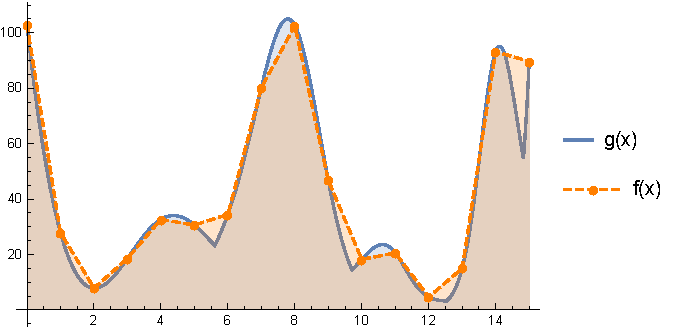
\includegraphics[width=8.5cm]{img_graph1}
	\end{center}
	\caption{La fonction $f(x)$ ou $h(x)$, relative à $g(x)$ et définie par $N=15$ points}
\end{figure}


\subsection{Échantillonnage uniforme avec variable de contrôle {\normalfont({\tt ControlSampler})}}

Cette dernière méthode d'échantillonnage est également une méthode de réduction de variance, dont l'objectif est de diminuer la variabilité des échantillons collectés pour réduire l'intervalle de confiance indépendamment du nombre d'itération effectuées.

Cette méthode requiert la connaissance d'une variable aléatoire $Z = h(X)$, fortement corrélée avec notre valeur à estimer $G$, dont l'espérance $\mu=E(Z)$ est connue.

Comme pour la méthode préférentielle, nous allons construire une telle variable en construisant une fonction affine-par-morceau $h(x)$ sur la base d'un découpage et échantillonnage régulier de la fonction $g(x)$. Idem, le nombre de tranches par défaut utilisé dans ce travail sera de $N=15$.

Cette méthode requiert en principe la conservation de chaque échantillon généré pour calculer le coefficient multiplicatif $c$. Il est cependant possible de se contenter d'une estimation de $c$ calculée sur un nombre restreint $M$ d'échantillons pour produire une constante $c$ qui sera \emph{assez bonne} pour produire des résultats de qualité satisfaisante.

Dans notre cas, nous utiliserons par défaut $M=10000$.

\subsection{Note concernant le paramètre $N$}

Le paramètre $N$ définissant le nombre de morceaux à construire lors de la fabrication des fonctions auxiliaires $f(x)$ ou $h(x)$ peut facilement être défini à une valeur \emph{trop élevée} et ne plus être cohérent avec l'objectif de ce laboratoire.

En effet, l'échantillonnage régulier de la fonction à intégrer avec beaucoup de précision peut conduire à des résultats pratiquement exactes avec un nombre d'itération minimal. Par exemple, en utilisant $N=100000$, il est possible de générer un intervalle de confiance de largeur $\Delta\text{IC} < 0.001$ en une seule itération de l'échantillonneur préférentiel.

Cependant, l'intérêt des méthodes de Monte-Carlo est d'être applicable sur un domaine d'intégration bien plus grand que $[0,15]$, là où l'échantillonnage haute résolution provoqué par un $N$ grand n'est plus envisageable.

C'est pourquoi nous nous limiterons ici à utiliser $N \le 15$.

\section{Validation des implémentations et performances pour un temps donné}

Avant de procéder à une analyse plus détaillée du comportement des différentes méthodes implémentées, il est nécessaire de s'assurer de leur bon fonctionnement. En tant que valeur de référence, j'ai choisi d'utiliser $G_W \approxeq 601.971$, calculée par WolframAlpha.

Chaque échantillonneur a ensuite été exécuté pendant 10 minutes, avant d'observer les résultats obtenus.
Le tableau de la figure 2 présente les résultats de cette première phase.

\begin{figure}[h]
\bgroup
\def\arraystretch{1.2}
\begin{center}
\begin{tabular}{|lcccccc|}
	\hline
	\textbf{Méthode} & \textbf{Itérations} & $\hat{G}$ & $\hat{\sigma}_{\hat{G}}$ & \textbf{IC$_{95\%}$} & \textbf{$\Delta$IC} & \textbf{$G_W \in$ IC}\\
	\hline
	Uniforme & $3.978 \cdot 10^9$ & 601.960 & 0.00713 & [601.946; 601.974] & 0.0280 & \cmark\\
	\hline
	Préférentiel & $2.863 \cdot 10^9$ & 601.973 & 0.00156 & [601.970; 601.976] & 0.0061 & \cmark\\
	$N=15$ & & & & & &\\
	\hline
	Variable de contrôle & $3.754 \cdot 10^9$ & 601.971 & 0.00281 & [601.968; 601.974] & 0.0056 & \cmark\\
	$N=15,M=10000$ & & & & & &\\
	\hline
\end{tabular}
\end{center}
\egroup
\caption{Résultats obtenus pour l'estimation de $G$ après 10 minutes d'exécution}
\end{figure}

\subsection{Analyse}

Aucune surprise ici, les trois échantillonneurs produisent une estimation de l'intégrale avec un intervalle de confiance contenant la valeur de référence et attestant ainsi leur bon fonctionnement.

Une analyse préliminaire confirme les attentes concernant les différentes propriétés de ces méthodes.

L'échantillonneur uniforme produit le plus grand nombre d'itérations dans un intervalle de temps donné, certainement due au fait de sa relative simplicité algorithmique par rapport aux deux autres. En revanche, l'intervalle de confiance qu'il produit est considérablement plus large que celui des deux autres méthodes, représentant ainsi un résultat de moins bonne qualité.

Les échantillonneurs préférentiel et avec variable de contrôle sont très similaires au niveau de la largeur de l'intervalle de confiance produit. Il est cependant intéressant de relever que l'écart-type de l'échantillonneur avec variable de contrôle est plus élevé que celui de l'échantillonneur préférentiel.

Il semblerait donc que les résultats produits avec variable de contrôle soient initialement moins précis. Cependant, sa vitesse d'exécution très proche de l'échantillonneur uniforme lui permet d'atteindre un nombre d'itérations bien plus élevé que l'échantillonneur préférentiel et produire ainsi un résultat équivalent, voir meilleur, que ce dernier.

\section{Performances pour un objectif donné}

Dans cette seconde phase, nous nous intéresserons à l'évolution du temps de calcul requis par chaque méthode pour atteindre une précision données, c'est à dire un intervalle de confiance dont la largeur ne dépasse pas un objectif fixé.

Le tableau de la figure 3 présente les résultats obtenus, illustrés par le graphique de la figure 4.

\begin{figure}[h]
\bgroup
\def\arraystretch{1.2}
\begin{center}
\begin{tabular}{|llccccc|}
	\hline
	\textbf{Objectif} & \textbf{Méthode} & \textbf{Temps} [s] & $\hat{G}$ & $\sqrt{N}\hat{\sigma}_{\hat{G}}$ & \textbf{IC$_{95\%}$} & \textbf{$\Delta$ IC}\\
	\hline
	                                  & Uniforme             & 1.8871 & 602.056 & 450.94 & [601.816; 602.306] & 0.4999\\
	$\Delta\text{\bfseries IC} < 0.5$ & Préférentiel         & 0.0962 & 601.882 & 83.287 & [601.633; 602.131] & 0.4979\\
	                                  & Variable de contrôle & 0.0886 & 601.972 & 88.188 & [601.722; 602.221] & 0.4990\\
	\hline
	                                   & Uniforme             & 7.6218 & 601.727 & 450.76 & [601.727; 601.977] & 0.2499\\
	$\Delta\text{\bfseries IC} < 0.25$ & Préférentiel         & 0.3602 & 601.988 & 83.126 & [601.863; 602.113] & 0.2499\\
	                                   & Variable de contrôle & 0.3143 & 601.989 & 88.079 & [601.864; 602.114] & 0.2498\\
	\hline
	                                    & Uniforme             & 30.200 & 602.017 & 450.85 & [601.955; 602.079] & 0.1249\\
	$\Delta\text{\bfseries IC} < 0.125$ & Préférentiel         & 1.4319 & 601.957 & 83.200 & [601.894; 602.019] & 0.1249\\
	                                    & Variable de contrôle & 1.2368 & 601.963 & 87.992 & [601.901; 602.025] & 0.1249\\
	\hline
	                                   & Uniforme             & 190.28 & 601.976 & 450.83 & [601.951; 602.001] & 0.0499\\
	$\Delta\text{\bfseries IC} < 0.05$ & Préférentiel         & 8.9191 & 601.962 & 83.150 & [601.937; 601.987] & 0.0499\\
	                                   & Variable de contrôle & 7.7002 & 601.966 & 87.979 & [601.941; 601.991] & 0.0499\\
	\hline
	                                    & Uniforme             & 759.29 & 601.966 & 450.83 & [601.954; 601.979] & 0.0249\\
	$\Delta\text{\bfseries IC} < 0.025$ & Préférentiel         & 35.625 & 601.974 & 83.147 & [601.962; 601.987] & 0.0249\\
	                                    & Variable de contrôle & 30.515 & 601.968 & 87.966 & [601.956; 601.988] & 0.0249\\
	\hline
\end{tabular}
\end{center}
\egroup
\caption{Résultats obtenus pour les mesures de temps ($N=15,M=10000$)}
\end{figure}

\begin{figure}[h]
	\begin{center}
		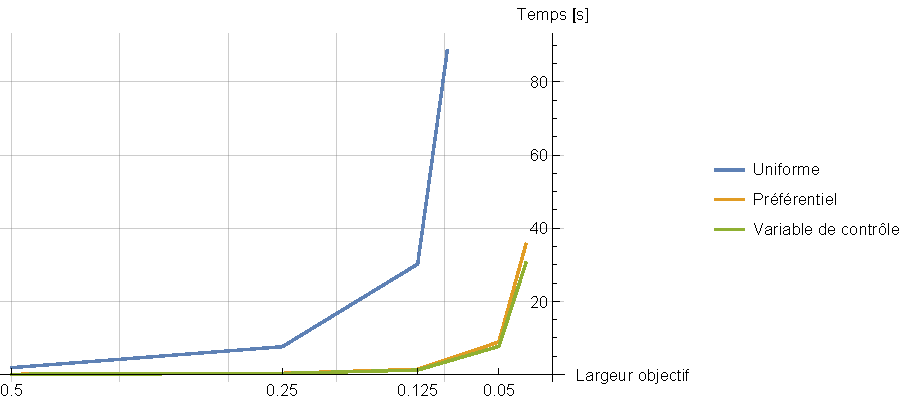
\includegraphics[width=15cm]{img_graph2}
	\end{center}
	\caption{Fonction $f(x)$ construite avec $N=15$ points}
\end{figure}

\subsection{Analyse}

À nouveau, les résultats obtenus ici sont conformes aux attentes et aux observations effectuées au point 3. Toutes les intervalles de confiance contiennent la valeur de référence $G_W$ et leur largeur correspond à l'objectif.

Globalement, les performances du générateur uniforme ne sont jamais compétitives avec celles des échantillonneurs préférentiels et avec variable de contrôle qui sont systématiquement plus de $20$ fois plus rapides à atteindre l'objectif. L'échantillonneur avec variable de contrôle est également toujours plus rapide que le préférentiel, mais dans une bien moindre mesure et les différences pratiques ne commencent à être humainement observables que lors d'une recherche d'intervalle dont la largeur est inférieure à $0.05$.

Une petite note concernant la variabilité de $\Delta\text{IC}$ pour les objectifs $0.5$ et $0.25$: idéalement, toutes ces valeurs devraient être les mêmes, juste en dessous de l'objectif puisque l'opérateur utilisé est strict. Cependant dans des soucis des performances, les test d'atteinte de l'objectif ne sont pas effectués toutes les itérations mais toutes les 10000 itérations.

Pour de grande valeurs d'itérations, cette particularité a un effet négligeable sur le résultat puisque celui-ci évolue de plus en plus lentement relativement aux itérations. À l'inverse, lorsque le nombre d'itération a effectuer pour atteindre l'objectif est faible, l'impact de l'exécution en bloc se manifeste de façon visible puisque la largeur de l'intervalle évolue alors beaucoup plus rapidement relativement au nombre d'itérations.

\section{Conclusion}

Les échantillonneurs implémentés dans le cadre de ce travail pratique semblent fonctionner de façon correcte et fournissent des résultats conforme aux attentes. 

Il est intéressant de constater la différence de performances, en terme de précision du résultat, entre une approche \emph{naïve} telle que celle de l'échantillonnage uniforme et des approches plus \emph{avancées} tel que les méthodes préférentielle et avec variables de contrôle. En pratique, l'implémentation des trois échantillonneur est très semblable, et le travail supplémentaire nécessaire au développement d'une approche \emph{avancée} peut pratiquement être considéré comme nul.

Ce laboratoire permet donc de se rendre compte qu'un bon développeur logiciel ne sait pas seulement résoudre les problèmes aux quels il fait face, mais qu'il sait les résoudre efficacement avec un effort équivalent... pour autant qu'il ait suivi ses cours avec attention ! :-)

\end{document}